\documentclass[final, size=a0]{beamer}
\usepackage{grffile}
\mode<presentation>
\usetheme{le2i}
\usepackage[english]{babel}
% \usepackage[latin1]{inputenc}
\usepackage{amsmath,amsthm, amssymb, latexsym}
\usepackage{multicol}
\usepackage{multirow}
\usepackage{algorithm}
\usepackage{algpseudocode}
\usepackage{latexsym}
\usepackage{xcolor}
\usepackage{epsf,graphicx,subfig}
\usepackage{epstopdf}
\usepackage{subfig}	
%% In order to draw some graphs
\usepackage{tikz,xifthen}
\usetikzlibrary{decorations.pathmorphing}
\usetikzlibrary{fit}
\usetikzlibrary{backgrounds}
\usetikzlibrary{shapes,arrows,shadows}
\usetikzlibrary{calc,decorations.pathreplacing,decorations.markings,positioning}
\usetikzlibrary{snakes,decorations.text,shapes,patterns}

\boldmath
\usepackage[orientation=landscape,size=a0,scale=1.4,debug]{beamerposter}
% change list indention level
% \setdefaultleftmargin{3em}{}{}{}{}{}
\usepackage[single=true, macros=true, xspace=true]{acro}

\usepackage{array,booktabs,tabularx}
\newcolumntype{Z}{>{\centering\arraybackslash}X} % centered tabularx columns
\newcommand{\pphantom}{\textcolor{ta3aluminium}} % phantom introduces a vertical space in p formatted table columns??!!

\usepackage{lipsum}
\usepackage{ragged2e}

\DeclareMathOperator*{\argmin}{arg\,min}
\DeclareMathOperator*{\argmax}{arg\,max}

\listfiles

%%%%%%%%%%%%%%%%%%%%%%%%%%%%%%%%%%%%%%%%%%%%%%%%%%%%%%%%%%%%%%%%%%%%%%%%%%%%%%%%%%%%%% 
\graphicspath{{images/}}

\title{\huge Normalization of T2W-MRI Prostate Images using Rician \textit{a priori}}
\author{G. Lema\^{i}tre, M. Rastgoo, J. Massich, J. C. Villanova, P. M. Walker, J. Freixenet, A. Meyer-Baese, F. M\'{e}riaudeau, and R. Mart\'{i}}
\institute[LE2I-UBFC / ViCOROB-UdG]{LE2I - Universit\'{e} de Bourgogne France-Comt\'{e} / ViCOROB - Universitat de Girona}
\date[February, 29th 2016]{February, 29th 2016}

% {Le2i-UMR CNRS 6306, BP 47870, 21078 Dijon, France\\
% Computer Vision and Robotics Group, Campus Montilivi, Edifici PIV, s/n, 17071 Girona, Spain}

%%%%%%%%%%%%%%%%%%%%%%%%%%%%%%%%%%%%%%%%%%%%%%%%%%%%%%%%%%%%%%%%%%%%%%%%%%%%%%%%%%%%%% 
\newlength{\columnheight}
\setlength{\columnheight}{91cm}

%% Acronym definition example using glossaries package
%% \usepackage{acro} is required
%% 
%% For a powerful usage of the acro package look at http://tex.stackexchange.com/questions/135975/how-to-define-an-acronym-by-using-other-acronym-and-print-the-abbreviations-toge

\DeclareAcronym{cad}{
  short = CAD, 
  long = Computer-Aided Diagnosis
}

\DeclareAcronym{rf}{
  short = RF,
  long = Random Forests
}

\DeclareAcronym{se}{
  short = SE,
  long = Sensitivity
}

\DeclareAcronym{sp}{
  short = SP,
  long =  Specificity
}

\DeclareAcronym{sift}{
  short = SIFT,
  long =  Scale-Invariant Feature Transform 
}

\DeclareAcronym{svd}{
  short = SVD,
  long =  Singular Value Decomposition 
}

\DeclareAcronym{pdf}{
  short = PDF,
  long =  Probability Density Function 
}

\DeclareAcronym{cap}{
  short = CaP,
  long =  Prostate Cancer 
}

\DeclareAcronym{mri}{
  short = MRI,
  long =  Magnetic Resonance Imaging 
}

\DeclareAcronym{pz}{
  short = PZ,
  long =  Peripheral Zone
}

\DeclareAcronym{cz}{
  short = CZ,
  long =  Central Zone
}

\DeclareAcronym{tz}{
  short = TZ,
  long =  Transitional Zone
}

\DeclareAcronym{trus}{
  short = TRUS,
  long =  Transrectal Ultrasound
}

\DeclareAcronym{psa}{
  short = PSA,
  long =  Prostate-Specific Antigen
}

\DeclareAcronym{pca}{
  short = PCA,
  long =  Principal Component Analysis
}

\DeclareAcronym{cg}{
  short = CG,
  long =  Central Gland
}

\DeclareAcronym{snr}{
  short = SNR,
  long =  Signal-to-Noise Ratio
}

\DeclareAcronym{rms}{
  short = RMS,
  long = Root Mean Square
}

\DeclareAcronym{auc}{
  short = AUC,
  long =  Area Under this Curve
}

\DeclareAcronym{srsf}{
  short = SRSF,
  long =  Square-Root Slope Function
}
      % contains the acronims


\setbeamercolor*{block body}{bg=azulunam!10!white,fg=niceblack}
\setbeamercolor*{block title}{fg=white,bg=blueubfc!70!white}
\setbeamerfont{block title}{size=\large,series=\bf}

\setbeamercolor*{block title example}{fg=white, bg=greenubfc!70!white}
\setbeamercolor*{block body example}{fg=niceblack, bg=azulunam!10!white}
\setbeamerfont{block title example}{size=\large,series=\bf}

\setbeamercolor*{block title alerted}{fg=white, bg=purpleubfc!70!white}
\setbeamercolor*{block body alerted}{fg=niceblack, bg=azulunam!10!white}
\setbeamerfont{block title alerted}{size=\large,series=\bf}

\setbeamertemplate{bibliography item}{\insertbiblabel}

\setbeamertemplate{caption}[numbered]

%%%%%%%%%%%%%%%%%%%%%%%%%%%%%%%%%%%%%%%%%%%%%%%%%%%%%%%%%%%%%%%%%%%%%%%%%%%%%%%%%%%%%% 
\begin{document}
\graphicspath{ {./images/article/} }
\begin{frame}
  \begin{columns}
    % ---------------------------------------------------------%
    % Set up a column 
    
    % ----------------------------------------------------------%
    % FIRST COLUMN 						  %
    % ----------------------------------------------------------%
    \begin{column}{.33\textwidth}
      \begin{beamercolorbox}[center,wd=\textwidth]{postercolumn}
        \begin{minipage}[T]{.95\textwidth}  % tweaks the width, makes a new \textwidth
          \parbox[t][\columnheight]{\textwidth}{ % must be some better way to set the the height, width and textwidth simultaneously
            % Since all columns are the same length, it is all nice and tidy.  You have to get the height empirically
            % ---------------------------------------------------------%

            % Introduction            
            \begin{exampleblock}{Introduction}
              \begin{itemize}
              \justifying
              \item \Ac{cap} has been reported the \textbf{second} most frequently diagnosed cancer of men accounting for 13.6\%~\cite{ferlay2010estimates}.
              \item \Ac{cad} systems have been proposed in order to assist the radiologists and generally consist of four stages: (i)~\textbf{\emph{pre-processing}}, (ii)~\emph{segmentation}, (iii)~\emph{registration}, and (iv)~\emph{classification}~\cite{Lemaitre2015}.
              \item \textbf{Normalization} is crucial to overcome the \textit{inter-patient} intensity variations, enforce the \textit{repeatability}, and achieve a \textit{robust} classification.
              \end{itemize}
            \end{exampleblock}
            
            \vspace{.5cm}

            % State-of-the-art methods
            \begin{exampleblock}{State-of-the-art method}
              \begin{itemize}
              \justifying
              \item Artan\,\textit{et al.}~\cite{artan2010prostate} and Ozer\,\textit{et al.}~\cite{ozer2010supervised} used the \emph{$z$-score} (see Eq.\,\eqref{eq:zscore}) to normalize T2W-MRI.
              \item Lv\,\textit{et al.}~\cite{lv2009computerized} and Viswanath\,\textit{et al.}~\cite{viswanath2012central} used methods based on piecewise-linear normalization~\cite{nyul2000new}.
              \end{itemize}
            \end{exampleblock}

            \vspace{.5cm}

            % Contributions
            \begin{exampleblock}{Contributions}
              \justifying
              We proposed two alternative methods:
              \begin{itemize}
              \justifying
              \item[(i)] a \emph{model-based} approach using Rician \textit{a priori};
              \item[(ii)] a \emph{non-parametric based} approach based on the \ac{srsf} representation~\cite{Srivastava2011}.
              \end{itemize}
            \end{exampleblock}

            \vspace{.5cm}

            % Comparison Rician Gaussian            
            \begin{alertblock}{Model-based normalization}
            
              \begin{figure}
                \centering
                \subfloat[][]{
                  \label{fig:p1}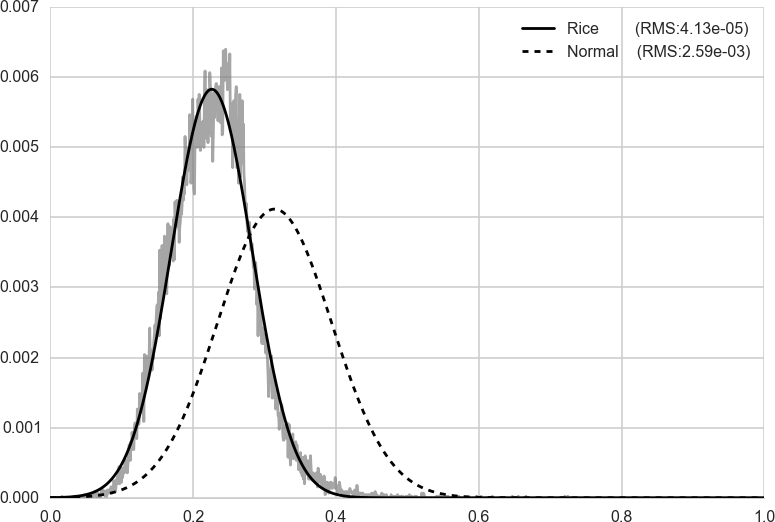
\includegraphics[width=0.48\textwidth]{03}}\hfill
                \subfloat[][]{
                  \label{fig:p2}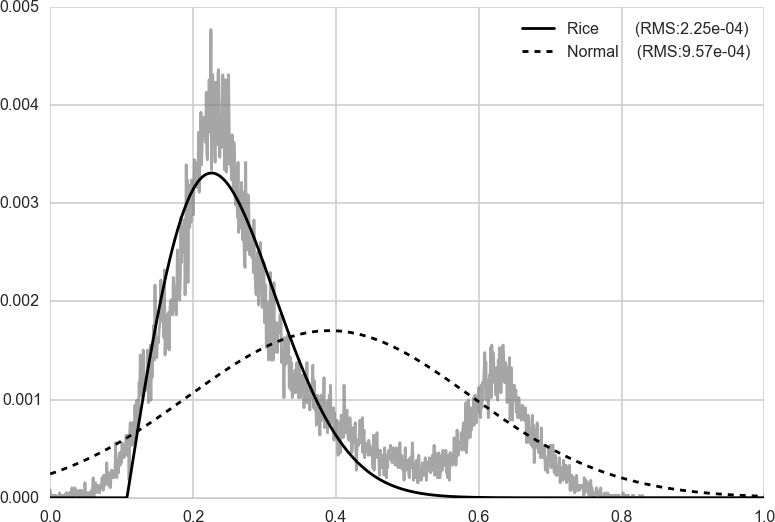
\includegraphics[width=0.48\textwidth]{06}}\hfill
                \caption{Visual evaluation of the goodness of fitting using Rician and Gaussian distribution.}
                \label{fig:fitting}
              \end{figure}

              \vspace{-.5cm}

              \begin{columns}
                \begin{column}{.5\textwidth}
                  
                  % Gaussian normalization
                  \begin{center}
                    \textbf{Gaussian normalization}
                  \end{center}

                \end{column}
                \begin{column}{.5\textwidth}
                  % Rician normalization
                  \begin{center}
                    \textbf{Rician normalization}
                  \end{center}
                \end{column}
              \end{columns}

              \vspace{1cm}

              \begin{columns}
                \begin{column}{.5\textwidth}
                  % Gaussian normalization
                  \begin{equation}\small
                    I_{s}(x) = \frac{I_{r}(x) - \mu_{G}}{\sigma_{G}} \ .
                    \label{eq:zscore}
                  \end{equation}
                \end{column}
                \begin{column}{.5\textwidth}
                  % Rician normalization
                  \begin{equation}\small
                    I_{s}(x) = \frac{I_{r}(x) - \mu_{R}}{\sigma_{R}} \ ,
                    \label{eq:zscorerician}
                  \end{equation}
                  \noindent where,
                  \begin{equation}\footnotesize
                    \mu_{R} = \sigma  \sqrt{\frac{\pi}{2}}\,\,L_{1/2}(-\frac{\nu^2}{2\sigma^2})  \ ,
                    \label{eq:meanr}
                  \end{equation}
                  \begin{equation}\footnotesize
                    \sigma_{R} = 2\sigma^2+\nu^2-\frac{\pi\sigma^2}{2}L_{1/2}^2\left(\frac{-\nu^2}{2\sigma^2}\right)  \ .
                    \label{eq:var}
                  \end{equation}
                \end{column}
              \end{columns}                
              \vspace{1cm}
              \begin{itemize}
              \justifying
              \item \acs{mri} data theoretically follows a Rayleigh distribution for a low \acs{snr} scenarios while it appears closer to a Gaussian distribution when the \ac{snr} increases~\cite{bernstein1989improved}.
              \item The Rician model better fits the data than the Gaussian model in terms of \acs{rms}.
              \end{itemize}

            \end{alertblock}
            
          }
        \end{minipage}
      \end{beamercolorbox}
    \end{column}
    % ----------------------------------------------------------------%
    % SECOND COLUMN                             % 
    % ----------------------------------------------------------------%
    \begin{column}{.33\textwidth}
      \begin{beamercolorbox}[center,wd=\textwidth]{postercolumn}
        \begin{minipage}[T]{.95\textwidth}  % tweaks the width, makes a new \textwidth
          \parbox[t][\columnheight]{\textwidth}{ % must be some better way to set the the height, width and textwidth simultaneously
            % Since all columns are the same length, it is all nice and tidy.  You have to get the height empirically
            % ---------------------------------------------------------%
            
            % Non-parametric normalization
            \begin{alertblock}{Non-parametric normalization}

              \begin{columns}
                % Piecewise-linear normalization
                \begin{column}{.5\textwidth}
                  \begin{center}
                    \textbf{Piecewise-linear normalization}
                  \end{center}
                \end{column}
                % SRSF-based normalization
                \begin{column}{.5\textwidth}
                  \begin{center}
                    \textbf{SRSF-based normalization}
                  \end{center}
                \end{column}
              \end{columns}
              
              \begin{figure}
                \centering
                \subfloat[][]{
                  \label{fig:piecewiselinear}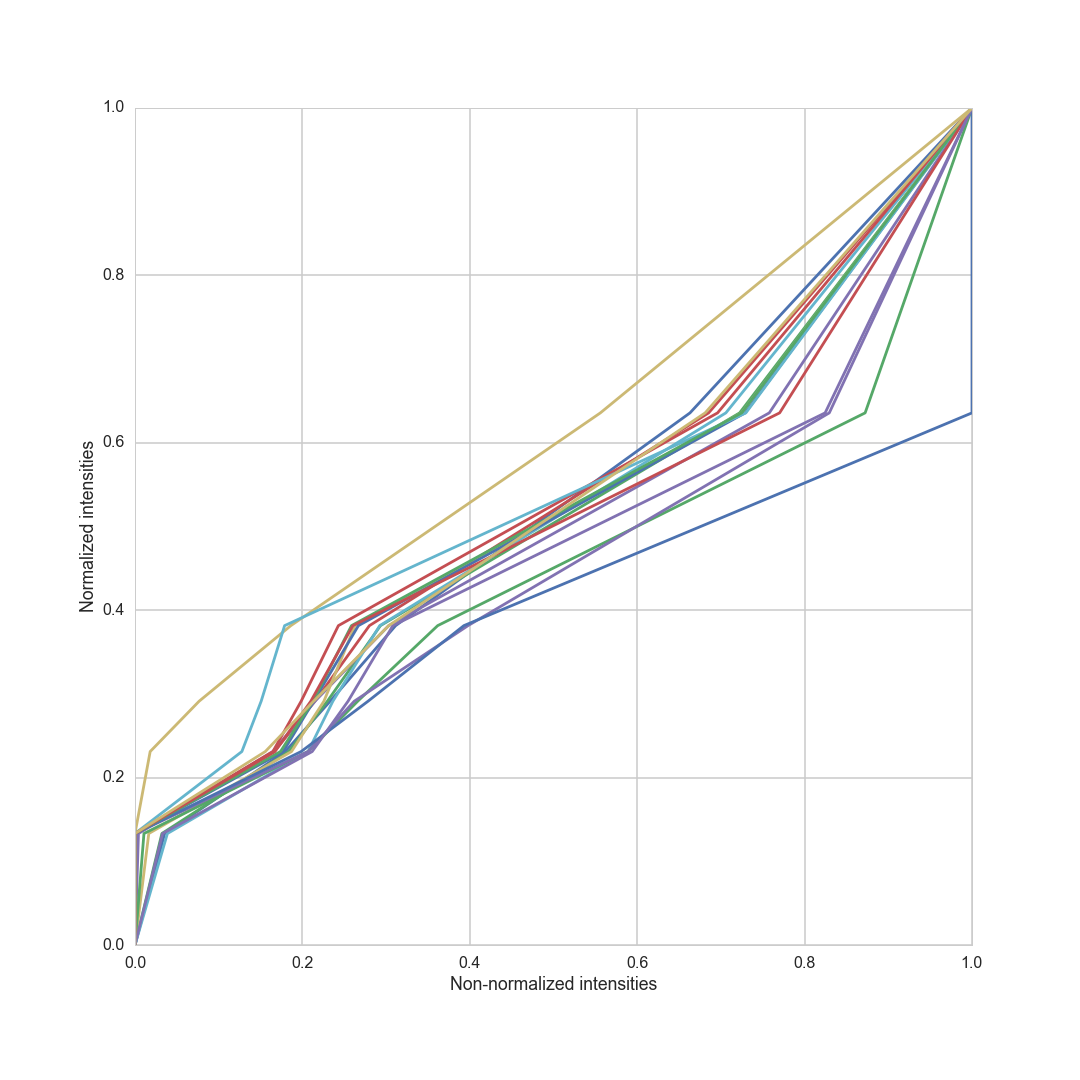
\includegraphics[width=0.48\textwidth]{piecewise-linear.png}}\hfill
                \subfloat[][]{
                  \label{fig:srsf}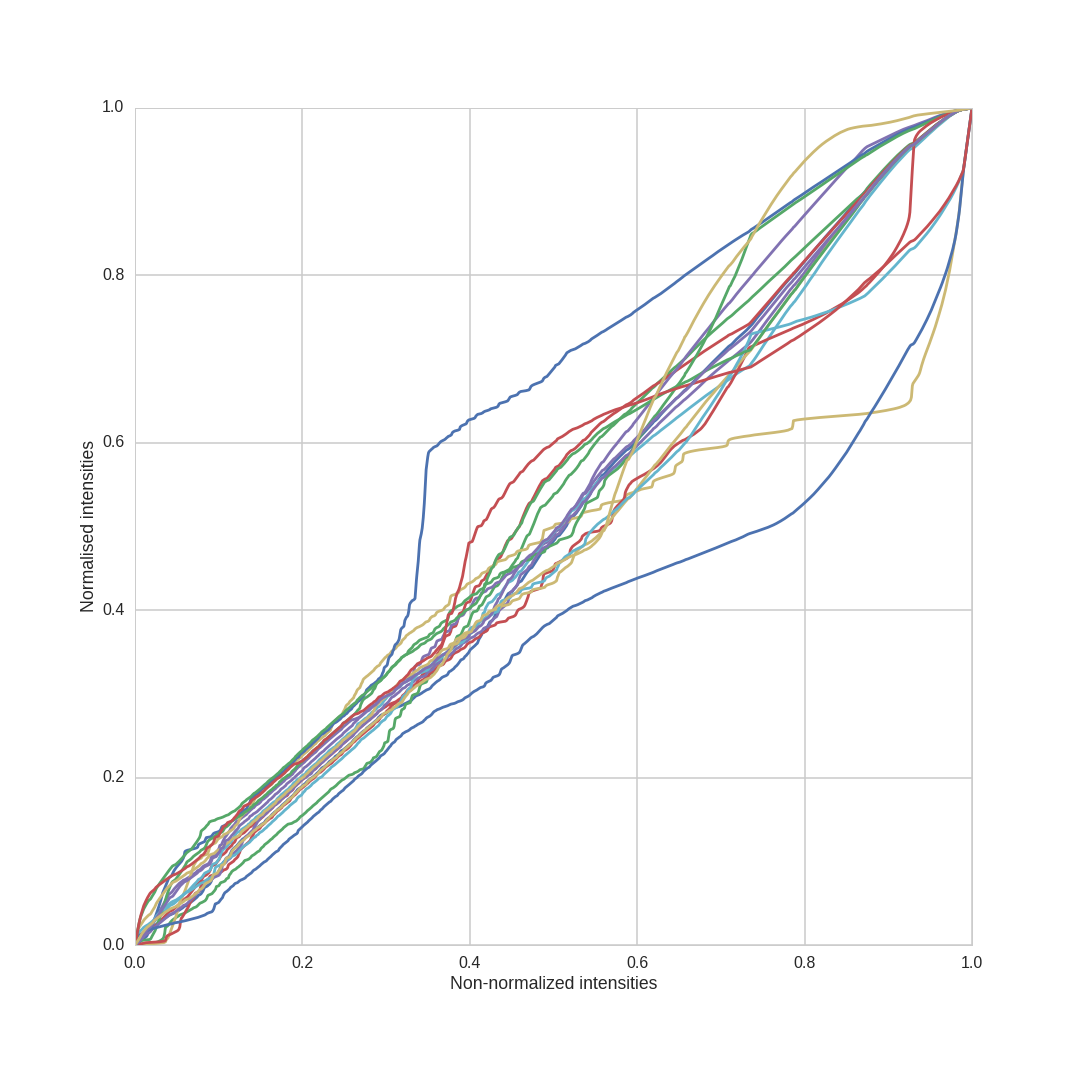
\includegraphics[width=0.48\textwidth]{srsf.png}}\hfill
                \caption{Comparison of warping function obtained with \protect\subref{fig:piecewiselinear} piecewise-linear normalization and \protect\subref{fig:srsf} \acs{srsf}-based normalization.}
                \label{fig:non-parametric}
              \end{figure}
              
              \begin{columns}
                \begin{column}{.5\textwidth}
                  % Piecewise-linear normalization
                  \begin{itemize}
                  \justifying
                  \item Minimize the distance between a set of standardized landmarks $\mu_i$ (i.e., atlas) and a set of non-normalized landmarks $\lambda_i$.
                  \end{itemize}
                \end{column}
                \begin{column}{.5\textwidth}
                  % Rician normalization
                  \begin{itemize}
                    \justifying
                  \item Minimize the distance between a mean \acs{pdf} $\mu_f$ (i.e., the Karcher mean) and a given patient \ac{pdf} $f_i$.
                  \end{itemize}
                \end{column}
              \end{columns}

              \vspace{1cm}

              \begin{itemize}
                \justifying
              \item \acs{srsf}-based normalization lead to smoother transition than piecewise-linear normalization.
              \end{itemize}

            \end{alertblock}

            \vspace{.2cm}

            % Dataset
            \begin{block}{T2W-MRI prostate dataset}
              \begin{itemize}
                \justifying
              \item 3 Tesla whole body MRI scanner.
              \item 17 patients manually segmented by experienced radiologist.
              \item Publicly available at \texttt{http://visor.udg.edu/i2cvb/}.
              \end{itemize}

            \end{block}

            \vspace{.2cm}

            % Quantitative results
            \begin{block}{Quantitative results}
              \begin{figure}
                \centering
                \subfloat[][]{
                  \label{fig:qtfull}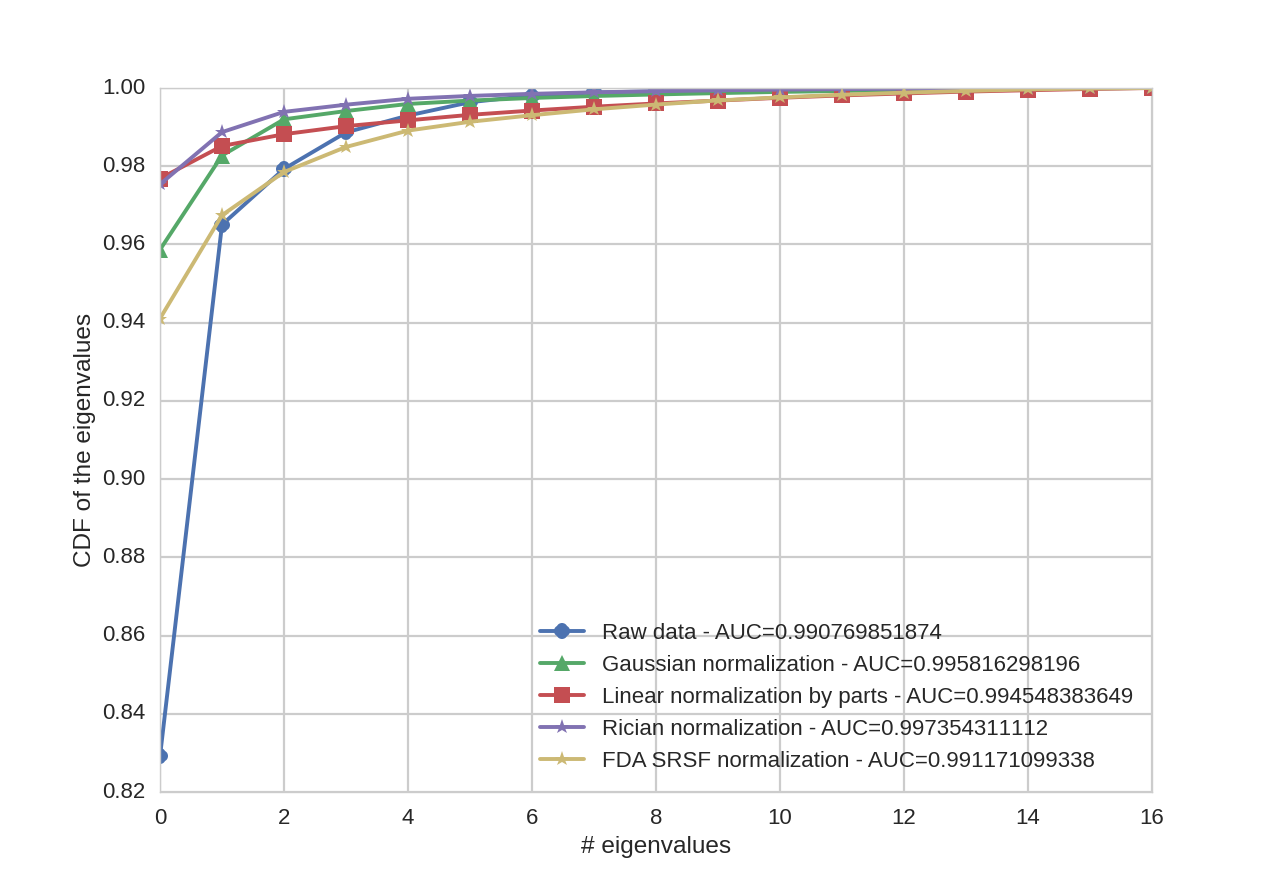
\includegraphics[width=0.48\textwidth]{quantitative_1.png}}\hfill
                \subfloat[][]{
                  \label{fig:qtcap}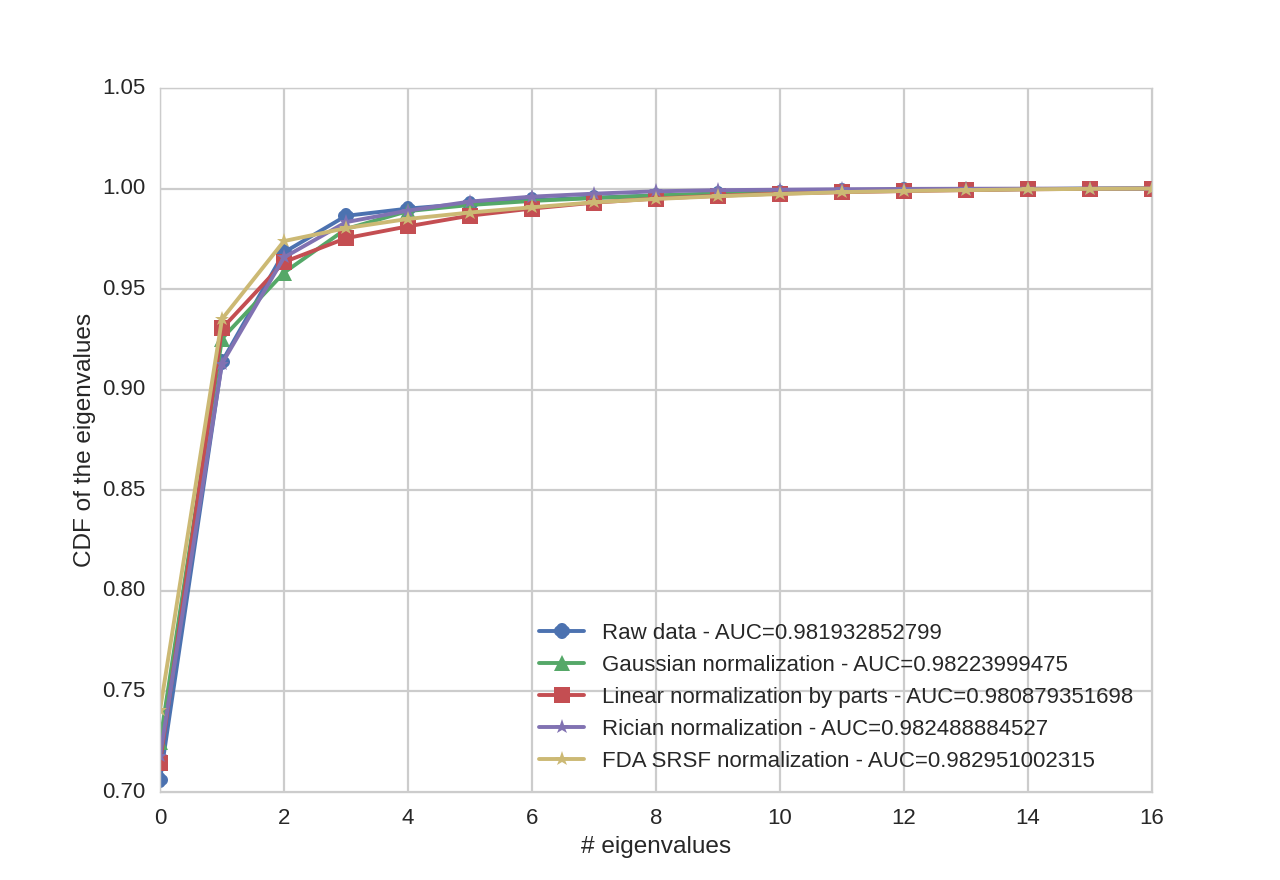
\includegraphics[width=0.48\textwidth]{quantitative_2.png}}
                \caption{Eigenvalue decomposition to evaluate the alignment of the \acs{pdf}s: \protect\subref{fig:qtfull} evaluation considering the full prostate, \protect\subref{fig:qtcap} evaluation considering only the \ac{cap}.}
                \label{fig:qt}
              \end{figure}
              
              \begin{itemize}
              \justifying
              \item Rician normalization outperforms the other methods: \ac{auc} of $0.9974$ and $0.9824$ considering the full prostate and \ac{cap}, respectively.
              \end{itemize}

            \end{block}
            
          }         
        \end{minipage}
      \end{beamercolorbox}
    \end{column}
    % ----------------------------------------------------------%
    % Third COLUMN 						  %
    % ----------------------------------------------------------%
    \begin{column}{.33\textwidth}
      \begin{beamercolorbox}[center,wd=\textwidth]{postercolumn}
        \begin{minipage}[T]{.95\textwidth}  % tweaks the width, makes a new \textwidth
          \parbox[t][\columnheight]{\textwidth}{ % must be some better way to set the the height, width and textwidth simultaneously
            % Since all columns are the same length, it is all nice and tidy.  You have to get the height empirically
            
            % Qualitative results
            \begin{block}{Qualitative results}
              \begin{figure}
                \centering
                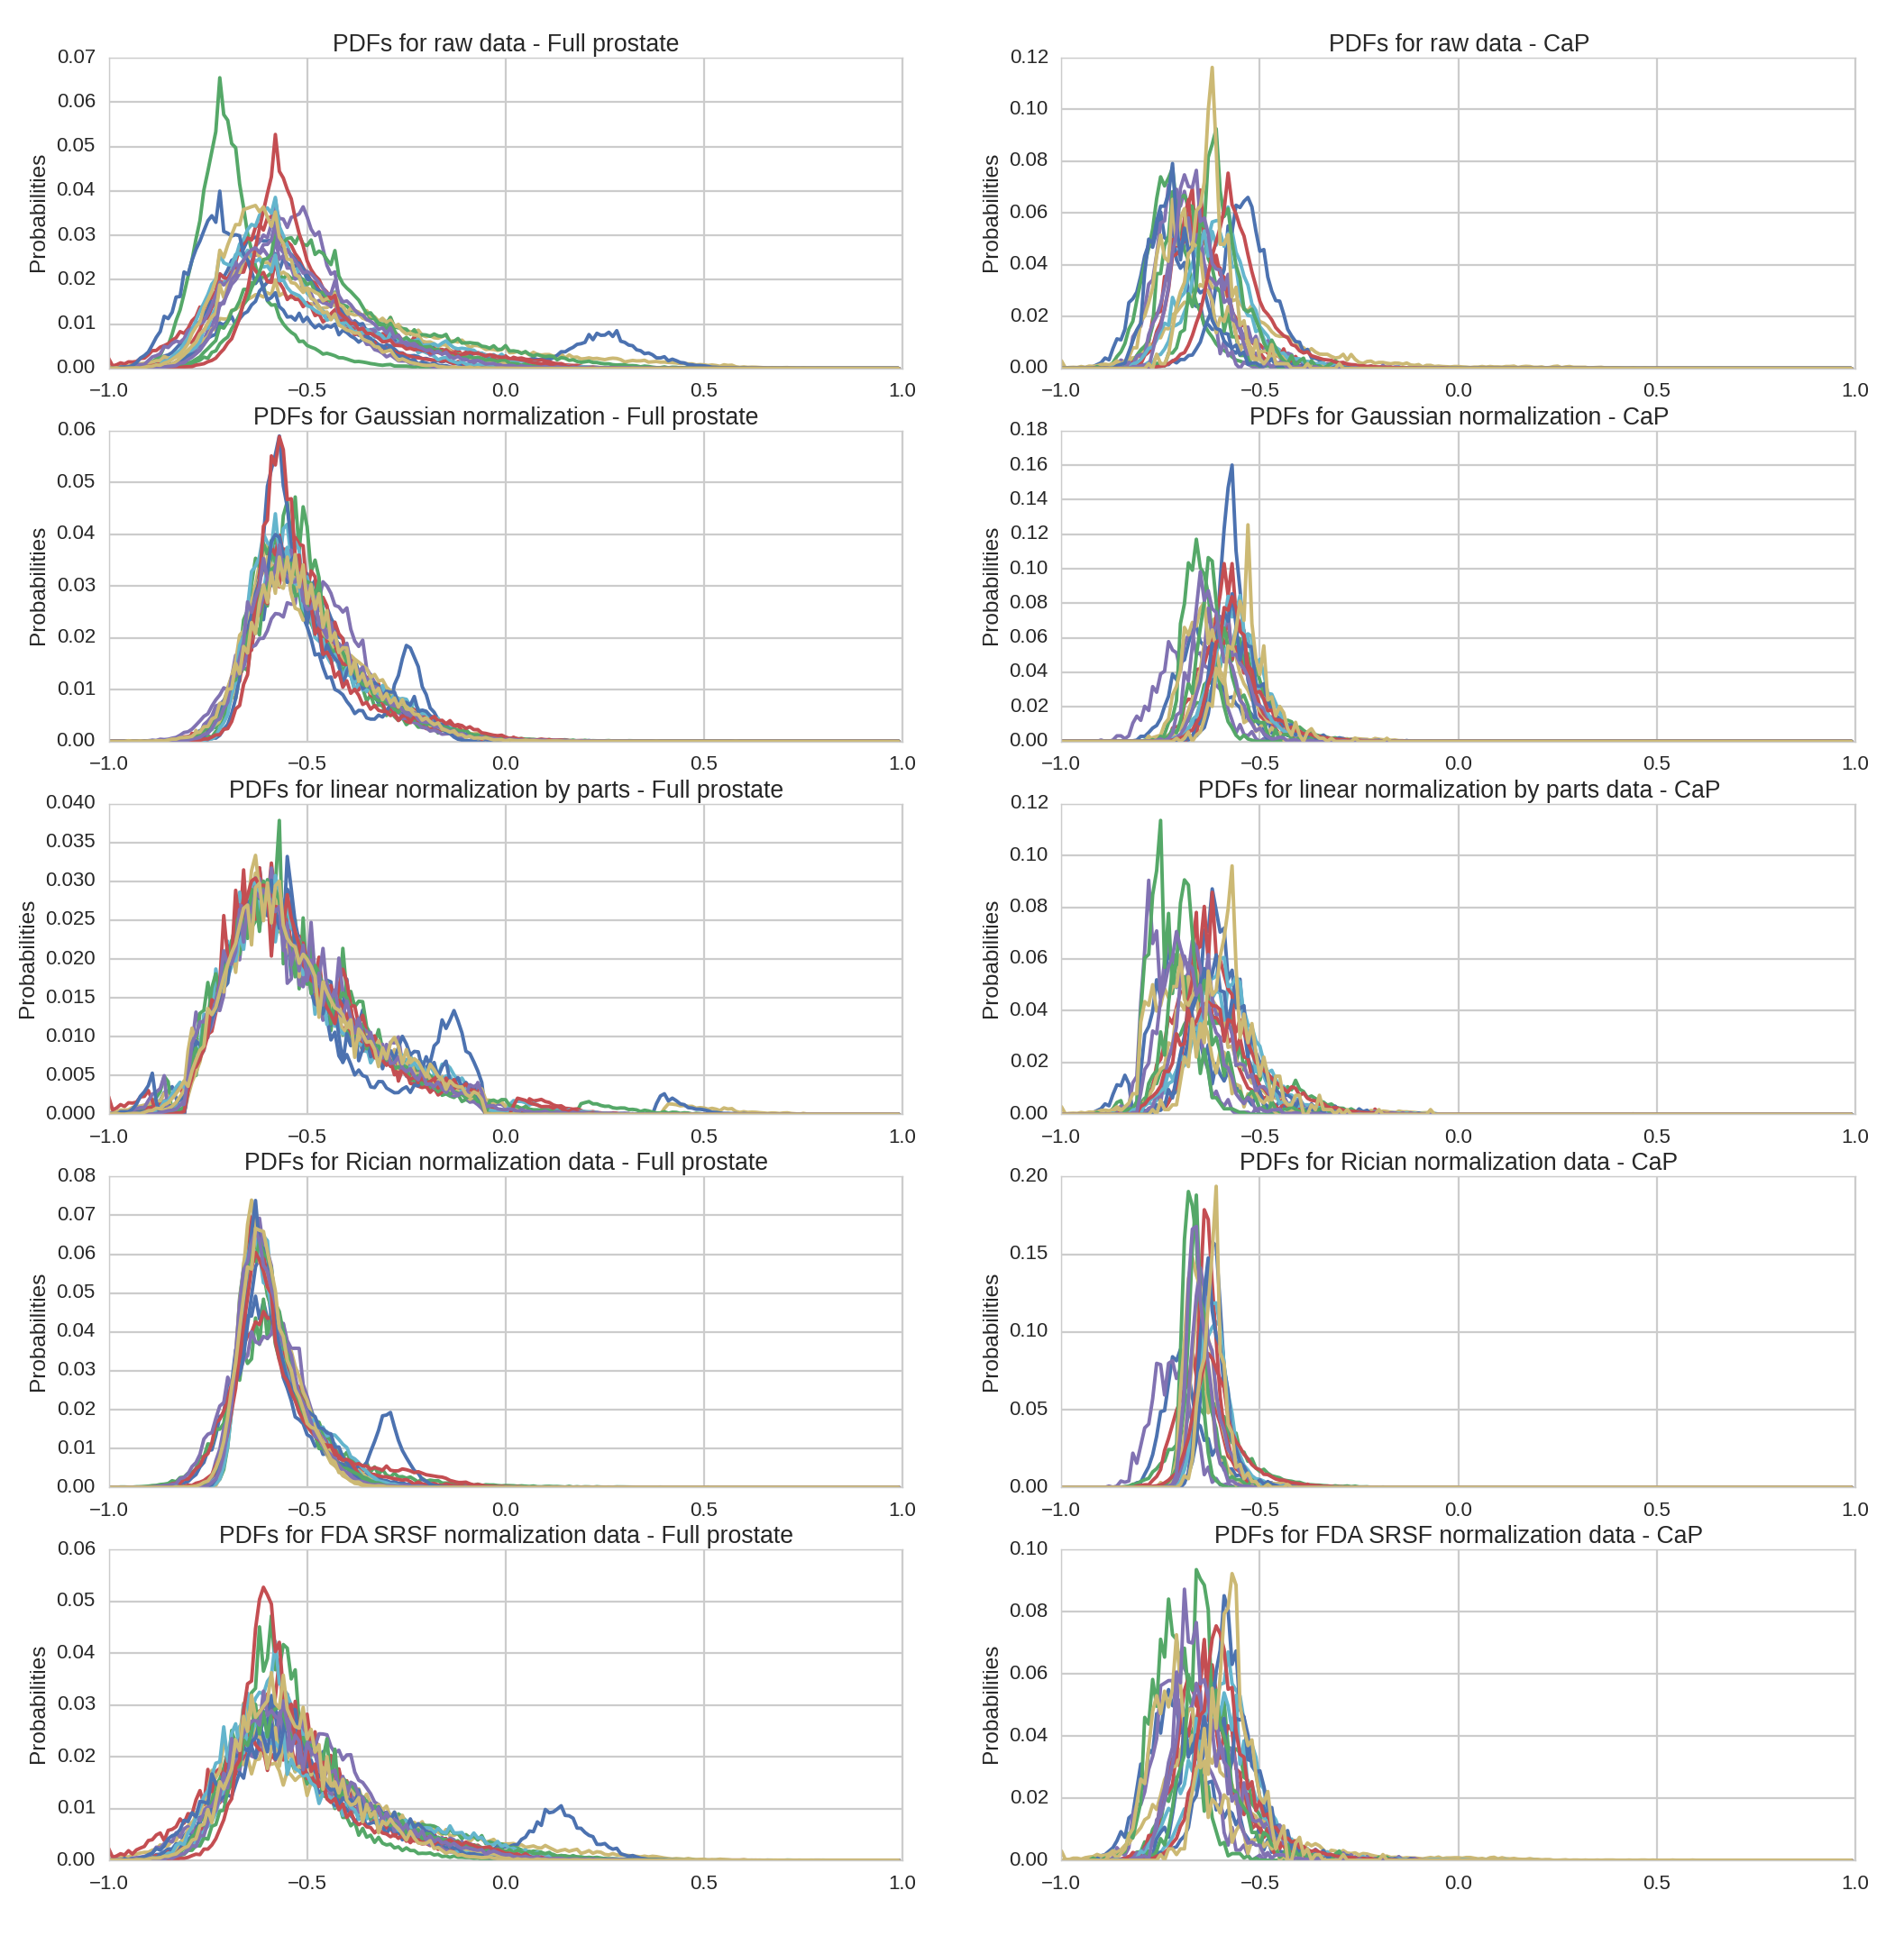
\includegraphics[width=1.\textwidth]{qualitative.png}
                \caption{Qualitative evaluation by visual inspection of the alignment of the \ac{pdf}s for the full prostate and the \ac{cap}.}
                \label{fig:qu}
              \end{figure}
              
              \begin{itemize}
              \justifying
              \item All the methods address the problem of the \ac{pdf} alignment of the full prostate data.
              \item However, the Rician normalization outperforms the other methods when focusing solely on the \ac{cap} data.
              \end{itemize}

            \end{block}

            % Conclusion
            \begin{exampleblock}{Conclusion}
              \justifying
              Comparisons show that the Rician normalization outperforms the Gaussian, \acs{srsf}-based, and piecewise-linear normalization for T2W-\acs{mri} prostate images normalization.
            \end{exampleblock}

            % \begin{block}{Acknowledgments}
            %   This work was supported by the Generalitat de Catalunya (grant nb. FI-DGR2012) and the Regional Council of Burgundy (grant nb. 2015-9201AAO050S02760).
            %   Calculations were performed using HPC resources from DSI-CCUB.
            % \end{block}

            % References
            \begin{exampleblock}{References}
              \renewcommand{\thepage}{}
              \tiny{\bibliography{literature_review}}
              \bibliographystyle{amsalpha}
            \end{exampleblock}

            
          }
        \end{minipage}
      \end{beamercolorbox}    

    \end{column}
    % ---------------------------------------------------------%
    % end the column
  \end{columns}
  \vskip1ex

  % \tiny\hfill\textcolor{ta2gray}{Created with \LaTeX \texttt{beamerposter}  \url{http://www-i6.informatik.rwth-aachen.de/~dreuw/latexbeamerposter.php}}
  % \tiny\hfill{Created with \LaTeX \texttt{beamerposter}  \url{http://www-i6.informatik.rwth-aachen.de/~dreuw/latexbeamerposter.php} \hskip1em}
\end{frame}

\end{document}


%%%%%%%%%%%%%%%%%%%%%%%%%%%%%%%%%%%%%%%%%%%%%%%%%%%%%%%%%%%%%%%%%%%%%%%%%%%%%%%%%%%%%%%%%%%%%%%%%%%% 
%%% Local Variables: 
%%% mode: latex
%%% TeX-PDF-mode: t
%%% TeX-master: t
%%% End:
